% Simple level diagram, resized and in a figure environment.
% Mark S. Everitt, 2009

\documentclass[10pt]{article}

% I only need the arrows for this one.
\usepackage{tikz}
\usetikzlibrary{arrows}

% Nice captions.
\usepackage[hang,small,bf]{caption}
\setlength{\captionmargin}{25pt}

% New commands to keep things tidy.
\newcommand{\ket}[1]{$\left|#1\right\rangle$}
\newcommand{\Om}[1]{\small $\omega_{#1}$}
\newcommand{\De}[1]{$\Delta_{#1}$}
\newcommand{\Ga}[1]{$\Gamma_{#1}$}



\begin{document}

\section{Feature branch workflow}

The life cycle of a feature branch is to be created from its tree, receive new commits, be merged back into its tree and finally be deleted.
The quality of the history reflected by the tree will depend on how easy it is to interpret the tree.
In general the more linear the easier to understand as a timeline where file changes have happened at distinct points in time by specific contributors.

The workflow can be visualized through Figure~\ref{fig:feature-happy-path}. 
During the simultaneous growth of the branch and the main tree there is potential for conflicts if the contributions made at the same location in the same file are different, technically the branch and the main tree have diverged.

\begin{figure}
    \centering
    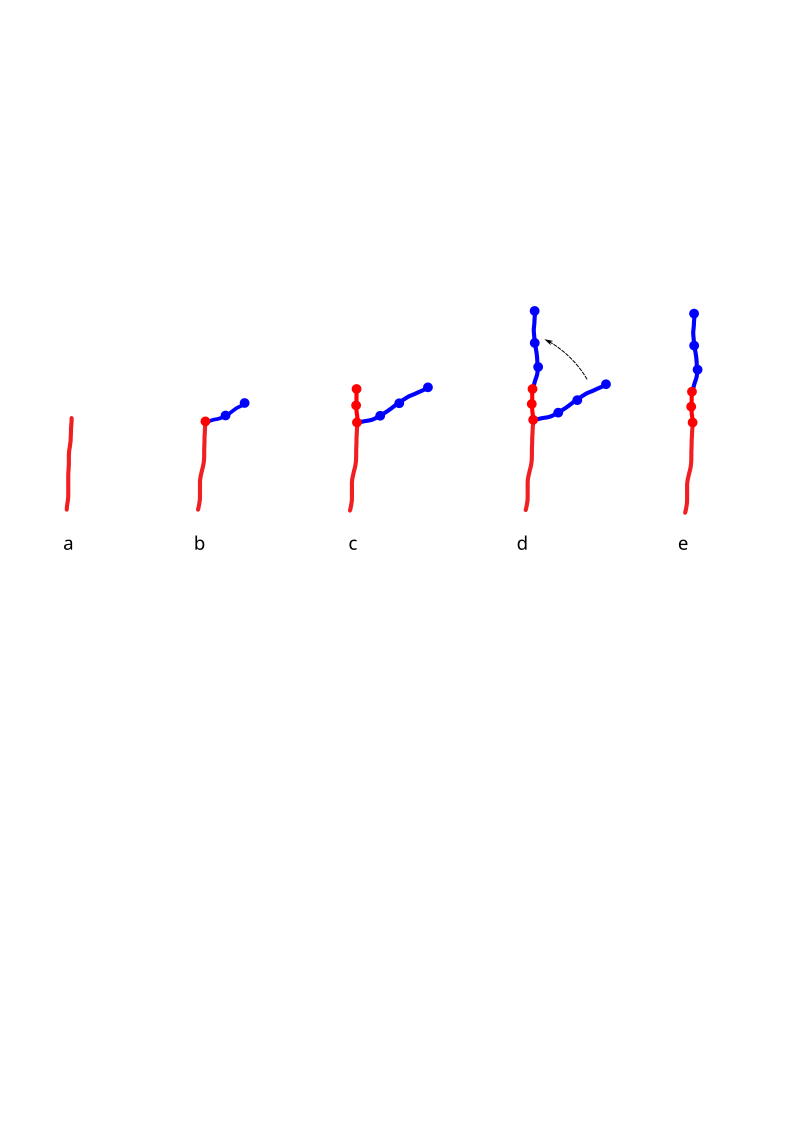
\includegraphics[width=\textwidth]{images/featurebranch_happy_path.png}
    \caption{Graphical representation of the history of a working tree when a feature branch is created. (a) The tree grows linearly, (b) the branch starts to grow, (c) both the branch and the main stem of the tree grow, (d) a copy of the branch is merged into the main stem, (e) the branch is removed.}
    \label{fig:feature-happy-path}
\end{figure}

In order to achieve this goal let's have a look at the best practice while using feature branches.
The workflow calls for two main git actions:

\begin{itemize}
    \item rebasing the source tree onto the feature branch as often as new commits appear on the source tree to address diverging histories.
    \item merging the feature branch into the source tree when the work is completed.
\end{itemize}

The first item, rebasing the source into the feature addresses potential conflicts created by the diverging timelines.




A feature branch \textit{feature} created from a \textit{dev} branch has to be rebased periodically with the purpose of minimizing and simplifying the conflicts later on if they occur while merging it into \textit{dev}.
The result will be a linear tree that is simple to read.

While working on the 

% Place the TikZ picture in a figure environment.
\begin{figure}
\centerline{
  % Resize it to 5cm wide.
  \resizebox{10cm}{!}{
    \begin{tikzpicture}[
      scale=0.5,
      level/.style={thick},
      virtual/.style={thick,densely dashed},
      trans/.style={thick,<->,shorten >=2pt,shorten <=2pt,>=stealth},
      classical/.style={thin,double,<->,shorten >=4pt,shorten <=4pt,>=stealth}
    ]
    % Draw the energy levels.
    \draw[level] (0cm,11em) -- (7cm,11em) node[right] {Main};
    \draw[level] (0cm,0em) -- (3cm,0em) node[right] {Dev};
    % \draw[level] (2cm,11em) -- (4cm,11em) node[midway,above] {\ket{b}};
    \draw[level] (0cm,-11em) -- (4cm,-11em) node[right] {Acc};
    % Draw the virtual levels.
    % \d1raw[virtual] (2cm,8em) -- (4cm,8em) node[midway,above] {\De{1}};
    % \draw[virtual] (4cm,-8em) -- (6cm,-8em) node[midway,below] {\De{2}};
    % \draw[virtual] (2cm,-5em) -- (0cm,-5em) node[midway,above] {\De{3}};
    % % Draw the transitions.
    % \draw[trans] (1cm,-2em) -- (2.5cm,8em) node[midway,left] {\Om{1}};
    % \draw[trans] (3.5cm,8em) -- (5cm,-8em) node[midway,right] {\Om{2}};
    % \draw[classical] (4.5cm,-8em) -- (1.5cm,-5em) node[midway,below] {\Ga{}};
    \end{tikzpicture}
  }
}
\caption{A level diagram with some transitions drawn in TikZ, resized,
                and placed in a figure environment.}
\end{figure}

\end{document} 
